% !TeX root = ../../thesis.tex
\chapter{Bayesian phylodynamics of SARS-CoV-2 in Pakistan}\label{ch:chapter2}

\begin{minipage}[b]{0.6\textwidth}
    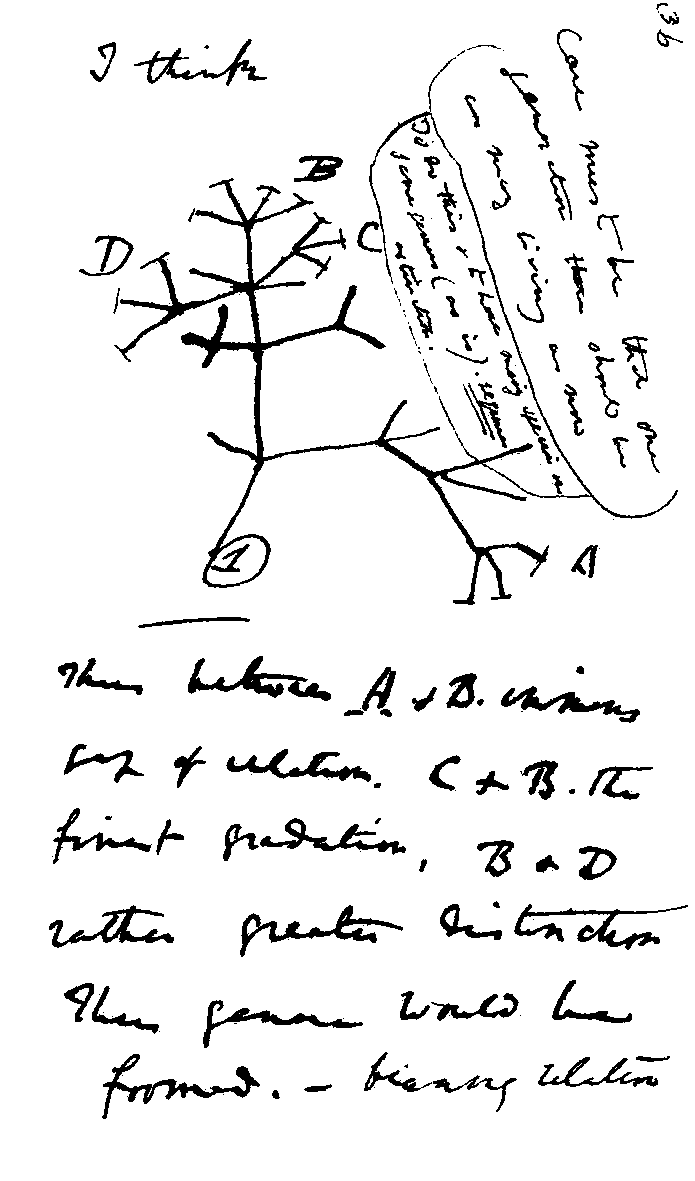
\includegraphics[width=\textwidth]{title} % Note: image needs to be cropped and faded
    % https://phil.cdc.gov/Details.aspx?pid=23312
  \end{minipage}
  \hfill
  \begin{minipage}[b]{0.32\textwidth}
    \footnotesize
    \begin{flushright}
      \textit{``A learning experience\\is one of those things that says,\\`You know that thing\\you just did?\\Don't do that.'\thinspace''} \\
      --- Douglas Adams, \\The Salmon of Doubt
    \end{flushright}
    \vspace{2cm}
\end{minipage}
  
\clearpage

\singlespacing

\hrule
\vspace*{12pt}
At the time of thesis submission, this chapter is in review at \textit{Journal of Medical Virology} as: \textbf{Barney I. Potter, Zaira Rehman, Muhammad Salman, Aamer Ikram, Samuel L. Hong, Gytis Dudas, Mandev S. Gill, Guy Baele, and Massab Umair.} Genomic epidemiology of Omicron (BA.1) as a driver of Pakistan's fifth SARS-CoV-2 wave."
I performed phylogenetic and phylogeographic analysis and wrote the manuscript.
Other authors contributed to the study design, data collection, and manuscript writing and editing.
\vspace*{12pt}
\hrule

\onehalfspacing

\section{Abstract}
The emergence of the SARS-CoV-2 Omicron variant led to Pakistan's fifth COVID-19 wave from December 2021 to March 2022.
This study investigates the molecular epidemiology of the early Omicron wave in Pakistan through genomic surveillance and travel history-informed Bayesian phylogeographic inference.
PCR-based genotyping and whole-genome sequencing show a shift from the BA.1 lineage's early replacement of Delta as Pakistan's dominant lineage in December 2021, until it was replaced by BA.2 predominance by March 2022.
We identify rare spike protein mutations and the absence of key mutations in circulating strains.
In order to determine the earliest drivers of the BA.1 wave in Pakistan we performed Bayesian phylogeographic analysis which revealed multiple introductions of BA.1 into Pakistan, primarily from Northern Europe.
Our findings highlight the importance of continued genomic surveillance, particularly at points of entry, and the need to address global disparities in sequencing capacity to better understand and control the spread of SARS-CoV-2 variants.


\section{Introduction}
The emergence and spread of novel variants fueled the persistence of the COVID-19 pandemic from its beginning in 2019 \cite{harvey2021sars, tao2021biological}.
The emergence of the Omicron (B.1.1.529, BA, and later XBB lineages) variant of concern (VOC) led to a large wave of COVID-19 cases worldwide, starting November 22, 2021.
This VOC featured advantageous mutations that boosted its fitness \cite{dhawan2022Omicron, francisco2022emergence} to the point where it displaced the Delta VOC, triggering a wave that quickly spread globally.
Its subsequent cryptic transmission severely impacted Pakistan, which first detected the variant on December 13, 2021.
Later, persistent local transmission caused a surge in the number of cases, resulting in the fifth wave of the pandemic, which spanned from mid-December 2021 to March 2022, with a peak positivity rate exceeding 12\% \cite{ourworldindataPK}.
Before the fifth wave, 1\,285\,254 severe cases of SARS-CoV-2 were reported in Pakistan, along with 28\,737 deaths.
Prior to the emergence of Omicron, Delta was the dominant VOC in Pakistan, and only 25\% of the total population was fully vaccinated \cite{covid-pakistan-stats}.
Moreover, it was found that that Omicron-infected patients had significantly higher vaccine breakthrough rates compared to Delta-infected patients \cite{christensen2022signals}.
In response to the emerging variants in Pakistan, it became necessary not only to curb the pandemic through vaccination but also to understand the dynamics of Omicron variants' evolution.

The Omicron VOC initially drew global attention due to its large number of mutational differences from the previously-dominant Delta VOC.
More than 30 mutations in the spike region altered its potential for transmission, replication proficiency and antibody binding \cite{viana2022rapid}.
Omicron demonstrated a capability to evade the immune response even with prior vaccination, with a subsequent risk of reinfection \cite{cele2022Omicron, lista2022p681h}.
Based on the genomic diversity of Omicron, five distinct lineages were reported: BA.1, BA.2, BA.3, BA.4 and BA.5 \cite{o2022pango}.
Lineage BA.1 spread globally, leading to new waves of infections in many countries, displacing the highly transmissible Delta soon after its initial detection \cite{yamasoba2022virological}.
After the emergence of BA.2 in February 2022, BA.1 was replaced by this more transmissible variant.
Globally, BA.2 constituted most of the sequences submitted to GISAID (961\,114), followed by BA.1 (502\,472) as of May 19, 2022.
BA.2 differed from BA.1 by 27 mutations \cite{wolter2022early}, notably with BA.2 lacking the S69/70 deletion, which could be screened in spike gene target failure samples using specific real-time PCR kits.
This lack of the S69/70 deletion, made it more difficult to detect using such real-time PCR kits.

We investigated the circulating variants of SARS-CoV-2 in Pakistan during the BA.1/BA.2 wave using a real-time PCR-based approach that was fast, economical, and could be used by labs in resource-limited settings.
We confirmed the PCR results through whole-genome sequencing and performed Bayesian phylodynamic inference on all samples that were confirmed as BA.1.
Here we describe how Omicron was responsible for the fifth wave of the pandemic in Pakistan, dominated by lineages BA.1, and BA.2, and their associated sublineages.
We use Bayesian phylogeographic inference informed by individual travel histories to understand the earliest origins of the fifth wave of Pakistan's SARS-CoV-2 epidemic, which came from lineage BA.1.
Through our analysis, we uncover that the driving force of the early BA.1 epidemic that started Pakistan's fifth wave was driven by travelers entering Pakistan from Northern Europe, with later introductions coming from around the globe.
Additionally, we find that the incoming travelers were a significant driver of the genetic diversity of BA.1 in Pakistan during this wave, with roughly half of the sequences we consider coming from independent introductions to Pakistan.
Our results underscore the force of incoming infection to Pakistan during the BA.1/Omicron wave from foreign countries; they also demonstrate the need for increased access to high-throughput sequencing in underrepresented countries to help understand and combat the dynamics of COVID-19 spread.


\section{Materials and Methods}\label{sec-mm}

\subsection{Sampling}\label{2:mm-sampling}
Between December 1, 2021 and April 10, 2022, oropharyngeal swab specimens of suspected subjects (25\,000) were collected as part of routine surveillance at the National Institute of Health's Department of Virology in Islamabad.


\subsection{RNA extraction and real-time PCR}\label{2:mm-pcr}
RNA extraction was performed using the MagMAX Viral/Pathogen Nucleic Acid Isolation kit (ThermoFisher Scientific, USA) and the KingFisher Flex instrument (ThermoFisher Scientific, USA).
Clinical RT-PCR testing was performed using the TaqPathTM COVID-19 RT-PCR kit (ThermoFisher Scientific, USA) on an Applied Biosystems 7500 Real-Time PCR system (Thermo Fisher Scientific, USA) that targets three genes (ORF1ab, N and S).
Based on spike gene amplification, the samples were divided into two categories: spike gene target failure (SGTF) and non-SGTF.
All the samples were further subjected to genotyping using the SNPsig\textsuperscript{\textregistered} SARS-CoV-2 (EscapePLEX) kit (PrimerDesign, UK) that targets K417N, E484K, and P681R mutations.
A subset of non-SGTF samples amplification of K417N was selected for whole-genome sequencing.


\subsection{cDNA synthesis and amplification }\label{2:mm-amp}
The cDNA synthesis and amplification were performed according to the ARTIC amplicon sequencing protocol (version 2) using SuperScript\texttrademark IV VILO\texttrademark Master Mix (Invitrogen, USA) and Q5\textsuperscript{\textregistered} High-Fidelity 2X Master Mix (New England BioLabs, USA), with the ARTIC nCoV-2019 Panel V3 (Integrated DNA Technologies, Inc, USA) \cite{quick2020ncov}.


\subsection{Next-generation sequencing}\label{2:mm-seq}
The paired-end sequencing library (2x150 bp) was prepared from the generated amplicons using the Illumina DNA Prep Kit (Illumina, Inc, USA) by following the standard protocol.
The prepared libraries were pooled and subjected to sequencing on the Illumina platform, iSeq using sequencing reagent, iSeq 100 i1 Reagent v2 (300-cycle) (Illumina, Inc, USA) at Department of Virology, National Institute of Health, Islamabad, Pakistan.


\subsection{Genome assembly and typing}\label{2:mm-assembly}
The Fastq files were processed for quality assessment using the FastQC tool (v0.11.9)\cite{andrews2010fastqc}.
Trimmomatic (v0.39) \cite{bolger2014trimmomatic} was employed to eliminate artifacts and technical biases by removing adapter sequences and low-quality base calls ($<30$).
The filtered reads were aligned using the Burrows-Wheeler Aligner's (BWA, v0.7.17) \cite{li2010fast} and available reference genome (Wuhan-Hu-1, GISAID ID: EPI\_ISL\_402125).
According to Centers for Disease Control and Prevention (CDC, USA) guidelines, variants were identified and consensus sequences for all genomes were generated \cite{paden2020rapid}.
Pangolin v4.0.5 and pangoLEARN v1.3 were used to classify the assembled genomes into Pango lineages \cite{o2021assignment}.


\subsection{Maximum-likelihood phylogenetic analysis}\label{2:mm-ml}
Initial maximum-likelihood (ML) phylogenetic analysis was performed using Nextstrain's standard protocol for analyzing SARS-CoV-2 genomes \cite{hadfield2018nextstrain}.
We first queried BLAST for all SARS-CoV-2 genome sequences most similar to our study's Omicron isolates (67), and obtained each hit's sequence from the GISAID database \cite{shu2017gisaid}. 
This resulted in a total of 160 sequences, including sequences from the current study. 
We used Augur---Nextstrain's phylodynamic toolkit---to cluster the sequences \cite{huddleston2021augur}.
We aligned the sequences to the Wuhan reference genome with MAFFT v7.470 \cite{katoh2002mafft}.
We estimated the initial maximum-likelihood phylogenetic tree using IQTREE v1.6.12 \cite{nguyen2015iq}, which used a generalized time-reversible (GTR) nucleotide substitution model \cite{tavare1986some, yang1994estimating, zharkikh1994estimation}.
Phylogenetic confidence was assessed using bootstrapping.
The raw tree was rooted using the reference genome Wuhan/Hu-1/2019 (GISAID ID: EPI\_ISL\_402125).
We employed TreeTime v0.8.1 to infer maximum likelihood branch lengths for the phylogenetic tree \cite{sagulenko2018treetime} and used auspice \cite{hadfield2018nextstrain} to visualize the resulting tree.


\subsection{Bayesian phylogeographic analysis}\label{2:mm-beast}
To infer the sources from which SARS-CoV-2 was imported into Pakistan during the fifth wave, we used BEAST v.1.10.5 \cite{suchard2018bayesian} to perform a discrete Bayesian phylogeographic analysis \cite{lemey2009bayesian} that incorporated information about travel histories of sequences from Pakistan \cite{lemey2020accommodating}.
With the focus on the initial sources of Omicron's introduction to Pakistan during the beginnig of its globalization in late-2021 and early-2022, our subsequent Bayseian phylogeographic was restricted to only consider BA.1 sequences.

We constructed a dataset that included all available BA.1 genomes from Pakistan (63) that were available on GISAID at the time.
These genomes were added to an alignment consisting of sequences from a contemporary analysis published on \verb|nextstrain.org| \cite{hadfield2018nextstrain}.
This process yielded an initial dataset of 3\,127 dated BA.1 sequences, which were aligned with Nextalign \cite{aksamentov2021nextclade}.
To refine the dataset prior to Bayesian phylogeographic analysis, we used IQ-TREE 2 \cite{minh2020iq} to infer an ML phylogeny according to an evolutionary model that featured a GTR substitution model with empirical nucleotide base frequencies and a FreeRate model with three categories to account for among-site heterogeneity \cite{yang1995space, soubrier2012influence}. We performed five independent replicates of this analysis using different starting seeds, and took the resultant tree with the highest likelihood to use as a starting tree for subsequent subsampling and Bayesian phylogenetic analysis.

We pruned all sequences from the ML phylogeny that were dated later than our latest sequence from Pakistan, thus removing all sequences dated later than April 15, 2022, as well as any sequences that did not belong to the BA.1 clade.
Finally, the ML phylogeny was processed using a ``cluster downsampling'' algorithm by which any clade with taxa belonging to a single location (except Pakistan) had one of its constituent sequences chosen at random to be retained, and the rest discarded \cite{hong2020search}.
This was justified since clades consisting solely of sequences from the same location do not bring any additional information on the discrete-state spread process we aim to infer.
This processing yielded a final BA.1 dataset of 1\,690 total genomic sequences with exact sampling dates and geographic metadata, which we subsequently realigned with Nextalign in preparation for Bayesian phylogeographic analysis in order to reduce any potential artifacts of downsampling.
Our dataset included sequences from around the globe, and were each given a discrete location designation based on a bespoke scheme of geographic partitioning whereby Pakistan and its immediate neighboring countries were considered as separate locations, each of the provinces of China for which we had data was considered as a discrete location, and more distant locations were combined by their UN geoscheme classification, yielding 32 discrete locations (Suppl.~Table~\ref{tab:locations}) \cite{unUNSDx2014}.
To account for sampling bias in our discrete phylogeographic reconstruction, we also included travel history designations according to the method of Lemey et al. 2020 \cite{lemey2020accommodating} for the 15 Pakistani sequences for which such data were available (Supplementary Table~\ref{tab:travel_histories}).

The evolutionary and spatiotemporal histories of BA.1 for our downsampled dataset were jointly inferred in a Bayesian framework using Markov chain Monte Carlo (MCMC) sampling as implemented in BEAST \cite{suchard2018bayesian}.
To assist in computation we ran analyses using high-performance GPU computation as implemented by the BEAGLE 3 library \cite{baele2019high,ayres2019beagle}.
To account for among-lineage evolutionary rate variation, we employed an uncorrelated relaxed molecular clock model with branch-specific rates drawn from a lognormal distribution \cite{drummond2006relaxed}.
We specified a skygrid phylogenetic tree prior \cite{gill2013improving} that posited a piecewise constant effective population size featuring 52 equally spaced change points between the most recent sampling time and April 15, 2021.
We employed a Hamiltonian Monte Carlo algorithm to efficiently sample skygrid model parameters \cite{baele2020hamiltonian}.
We assumed an HKY nucleotide substitution model \cite{hasegawa1985dating}, and used a discretized gamma distribution model for among-site rate heterogeneity with four different rate categories \cite{yang1994maximum}.
We combined samples from eight independent MCMC simulations that were run for $6\times10^8$ iterations, and we verified adequate convergence and mixing with Tracer v1.7 \cite{rambaut2018posterior} after removing $\geq10\%$ of each Markov chain's samples burn-in.
We used the combined samples to approximate the posterior distribution and created maximum clade credibility (MCC) summary trees using TreeAnnotator v1.10 \cite{suchard2018bayesian}.
The resulting MCC trees were visualized in baltic v.0.2.0 (\url{https://github.com/evogytis/baltic}; accessed on July 18, 2023).


\section{Results}\label{2:sec-res}
During the study period, a total of 1\,642 samples tested positive for SARS-CoV-2 on real-time PCR using the TaqPath\texttrademark\ COVID-19 kit (ThermoFisher Scientific, USA).
Among these, 494 (30\%) samples showed the amplification of all three genes (ORF, N and S) (non-SGTF), whereas 1\,148 (69.9\%) samples had the spike gene target failure (SGTF) i.e., S69/70 deletion.
The SARS-CoV-2 genotyping assay (SNPsig EscapePLEX) showed that all 1\,642 samples had the K417N mutation whereas E484K, K417T and P681R mutations were not detected (Fig.~\ref{fig:genotyped}).
The samples with SGTF (S69/70 deletion) and K417N were termed as probable BA.1 (incl. sublineages) while samples with non-SGTF, presence of K417N and absence of E484K as probable BA.2 (incl. sublineages), based on the fact that 6S9/70 deletion along with K417N is found in only BA.1, whereas K417N alone is a characteristic mutation of BA.2.
Because the SARS-CoV-2 Beta VOC was no longer circulating by the end of 2021 the detection of K417N and absence of E484K could be used as a screening method for BA.2.
This finding was also confirmed through whole-genome sequencing where a subset of PCR-based BA.1 probable samples (57/163) and BA.2 probable samples (106/163) were accurately detected as BA.1 and BA.2 (incl. sublineages), respectively.

\begin{figure}[ht]
   \centering
   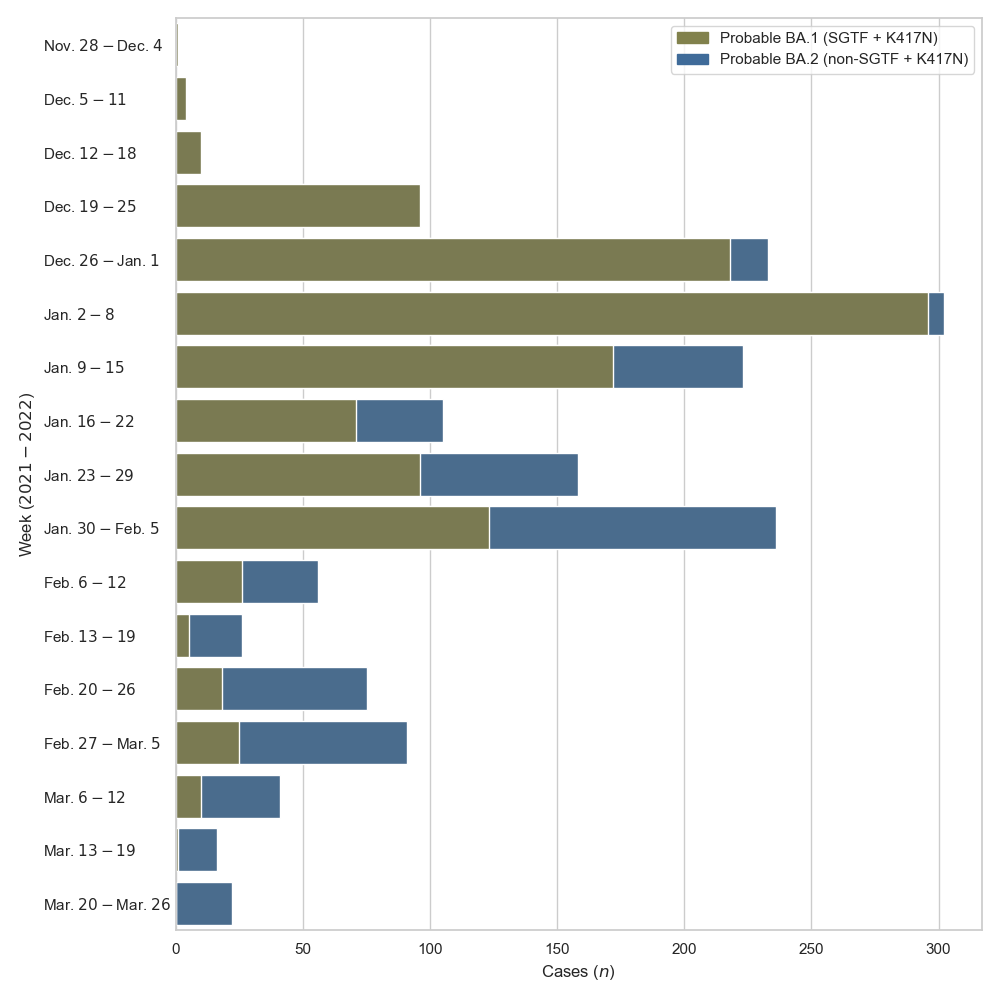
\includegraphics[width=0.45\textwidth]{case_counts_by_week.png}
    \caption{Weekly genotyping data of COVID-19 positive cases between December 1, 2021, and April 15, 2022 throughout Pakistan. The SGTF samples with K417N amplification are classified as probable BA.1 while non-SGTF with K417N amplification as probable BA.2.}
    \label{fig:genotyped}
\end{figure}

Based on whole-genome sequencing, two major descendants of Omicron (incl. sublineages), BA.1 (57/163; 34.97\%) and BA.2 (106/163; 65.0.\%), were identified from Pakistan (Fig.~\ref{fig:sublineages}).
The monthly distribution of Omicron sublineages showed the detection of the first case of BA.1 sublineage, BA.1.13 on December 3, 2021.
The most prevalent lineages in December 2021 were BA.1 (33\%), BA.1.17.2 (29\%), and BA.1.15.1 (19\%).
However, in January 2022, BA.1 declined to 14\%, BA.1.17.2 to 14\%, and BA.1.15.1 to 0\%.
There was also an emergence of new sublineages of Omicron, BA.1.1 (25\%) and BA.2 (41\%), January 2022.
The first case of BA.2 was reported on January 6, 2022, and there were subsequent changes in prevalence from 41\% to 80\% in February 2022, to 97\% in March 2022 and 93\% in April 2022.
Other BA.2 sublineages include BA.2.2 (3\%) in March 2022 and BA.2.1 (7\%) in April 2022 (Fig.~\ref{fig:sublineages}).

\begin{figure}[ht]
   \centering
   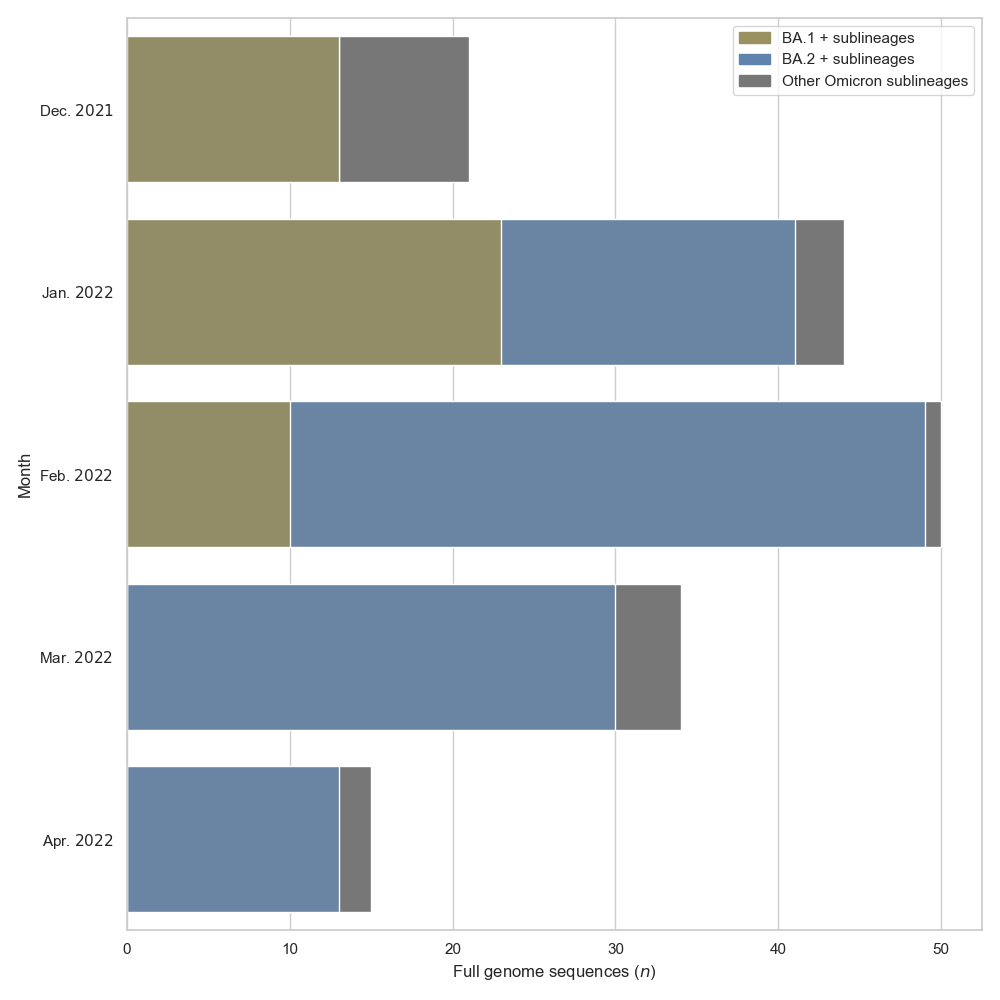
\includegraphics[width=0.45\textwidth]{sequences_by_month.png}
    \caption{Monthly distribution of BA.1, BA.2, and other Omicron sublineages which resulted in full-genome sequences in Pakistan between December 2021 and April 2022.}
    \label{fig:sublineages}
\end{figure}

% \begin{figure}[ht]
%    \centering
%    \includegraphics[width=0.45\textwidth]{images/pk-sublineage-heatmap.png}
%     \caption{Heatmap representing month-wise distribution of Omicron sublineages between December 2021, and April 10, 2022, based on whole-genome sequencing.}
%     \label{fig:heatmap}
% \end{figure}

%GB: not a fan of constantly using $n$ but I've stopped correcting them, I'll let you decide % bp: This was the nomenclature of the coauthors and their section, so I'm content with it being there
Among Omicron sublineages, Islamabad ($n=93$) reported the highest number of BA.2 cases ($n=68/93, 73.12\%$) compared to BA.1.17.2 ($n=8/93, 8.60\%$) and BA.1 ($n=7/93, 7.53\%$).
Furthermore, in Azad Jammu \& Kashmir ($n=26$), 19 cases of BA.2 sublineage ($73.08\%$) were reported compared to BA.1 ($n=4, 15.38\%$) and BA.1.1 ($n=3, 11.54\%$).
Khyber Pakhtunkhwa also reported primarily cases of BA.2 ($n=13/15; 86.67\%$) and one case each of BA.1 and BA.1.1 ($n=1/15, 6.67\%$).
In Gilgit Baltistan, the higher number of cases reported were of BA.1 ($n=4/11, 36.36\%$) and BA.1.1 ($n=4/11, 36.36\%$) compared to BA.2 ($n=3/11; 27.27\%$).
One case each of BA.1.13 and BA.1.1 was found in Sindh and Punjab, respectively (Suppl.~Table~\ref{tab:travel_histories}).
Sixteen patients (9.8\%) were reported to have an international travel history with highest number of cases from UK ($n=5/16; 31.25\%$) including most prevalent sublineages BA.1.1.14 ($n=2/5; 40\%$), BA.1.17.2 ($n=2/5; 40\%$), BA.1 ($n=1/5; 20\%$) and Ethiopia ($n=3/16; 18.75\%$) with all cases of BA.1.1 ($n=3/3; 100\%$).
The remaining countries included one case each from South Africa (BA.1), USA (BA.1.1), Maldives (BA.1.1), Turkey (BA.2), UAE (BA.1.17.2), Oman (BA.1.18), Congo (BA.1.17.2), and Saudi Arabia (BA.1.1) (Suppl.~Table~\ref{tab:travel_histories}).

%GB: I don't understand why you are dedicating a whole paragraph - and discuss results - on an initial ML tree ... won't the BEAST run still affect the topology?
% To determine the origin of the Pakistani isolates, we constructed a maximum-likelihood phylogenetic tree using 160 full-length genomes of SARS-CoV-2 viruses, including the high quality genomes from the current study ($n=67$).
% The Omicron sublineages detected in the current study shared significant similarities with isolates from Asia, Europe, North America, and Oceania.
% The BA.1 sublineage of Omicron clustered mostly with sequences from France, Germany, Canada, the USA, Denmark, and Australia.
% The isolates from travelers from the UK (GISAID ID: EPI\_ISL\_8240498, EPI\_ISL\_8240500, and EPI\_ISL\_8650048) infected with the BA.1 sublineage were genetically similar to lineages circulating in the USA and Denmark.
% Furthermore, sequences of travelers from Oman (EPI\_ISL\_8240501) and South Africa (EPI\_ISL\_8240513) were closely associated with viral sequences from France and Germany, and those from inbound passengers from Congo (EPI\_ISL\_8650053) and UAE (EPI\_ISL\_8824738) shared significant homology with viral isolates from Australia, Canada, and Denmark.
% The BA.1 cases reported in the current study were closely homologous with strains of Germany, USA, India, and Belgium.
% Among travelers, the BA.1.1 was detected mostly from passengers traveling from the UK (EPI\_ISL\_8824737 and EPI\_ISL\_8824739) with sequences clustering within the existing diversity of USA and Germany, and Ethiopian passengers (EPI\_ISL\_8824741, EPI\_ISL\_8824743, and EPI\_ISL\_8824745) whose sequences clustered with those from Germany, India, and Belgium.
% The BA.2 infected patient (EPI\_ISL\_8824736) had a travel history to Turkey and exhibited close homology with strains from Denmark and Belgium (Suppl.~Table~\ref{tab:travel_histories}).
% Our findings suggest multiple SARS-CoV-2 importations into Pakistan, as well as evidence of clustered outbreaks and community transmission, which we explored in our Bayesian phylogeographic analysis. %GB: but why not a single analysis instead of both ML and BEAST???

% \begin{figure}[ht]
%    \centering
%    \includegraphics[width=0.45\textwidth]{images/sublineage-dist.png}
%     \caption{Geographic distribution of Omicron sublineages reported in the current study.}
%     \label{fig:sl-dist}
% \end{figure}

%GB: in my opinion, you need to work on the flow of the Results section; first you discussed sequencing results, then phylogeny and now mutations, then breakthrough infections and then phylodynamics; you should group the sections according to topic
% The mutation profile of different sub-lineages of BA.1 has shown that all the isolates harbor characteristics mutations in the ORF1ab (NSP3:K38R, NSP3:S1265del, NSP3:A1892T, NSP4:T492I, NSP5:P132H, NSP6:LSG105/107del, NSP6:I189V, NSP12:P232L, NSP14:I42V), Envelope (T9I), Membrane (D3G, Q19E, A63T) nucleocapsid (P13L, ERS31/33 del, R203K, G204R) (Fig.~\ref{fig:thist} \bip{UPDATE THIS TO A TABLE APPROPRIATELY}).
% In the spike protein, a total of 31 substitutions, 6 deletions, and three amino acid insertion (ins214EPE) were observed (Table 1 \bip{What is going on here? Fix to a link}). %GB: would a figure be better than a table?
% In the spike protein, we have some interesting findings, in 8 of the isolates we don’t have a T95I mutation.
% Interestingly, the R346K and S375F mutations were not observed in 23 and 30 isolates, respectively.
% Moreover, in 8 of the isolates, we do not observe the Q498R, N501Y, and Y505H mutations.
% In addition to these, 11 isolates don’t exhibit the Y505H mutation. All of the BA.2 isolates exhibit the characteristic BA.2 mutations in the ORF1ab (NSP1:S135R, NSP3:T24I, NSP3:G489S, NSP4:T492I, NSP4:L264F, NSP4:L438F, NSP4:T327I, NSP5:P132H, NSP6: SGF106/108del, NSP12:P232L, NSP13:R392C, NSP14:I42V, NSP15:T112I), NS3 (T223I), membrane (Q19E, A63T), nucleoprotein (P13L, R203K, G204R, S413R, ERS31/33del) and envelope (T9I) protein (Fig.~\ref{fig:thist} \bip{TABLE}).
% In one of the isolates, an unusual stop codon (Q18stop) was observed in the NS8 protein.
% In the spike protein, a total of 28 mutations and three deletions have been identified (Table 2 \bip{gytis figure}).
% In comparison with the reference BA.2 mutations, the 42 study isolates did not exhibit the Y505H mutations.
% One of the isolates (EPI\_ISL\_12055219) did not exhibit 24/26del while in another isolate we did not observe S477N, T478K, and E484A.
% Interestingly, only five spike unique mutations were present in samples infected with BA.1.1 (D1163Y), BA.1.13 (T76I), BA.1.17.2 (F643L), and BA.2 (A783V, P1162L) variant.
% Moreover, there were also three rare spike mutations present in the study samples that are A264S ($n=2$), A701V ($n=5$), and D1153Y ($n=3$).

The vaccination status of sequenced individuals ($n=163$) infected with Omicron showed 58 to be fully vaccinated, 10 to be unvaccinated, and 95 to have unknown status.
Among fully vaccinated ($35.5\%, n= 58$) individuals, 37.9\% ($n=22$) received Sinopharm, 32.7\% ($n=19$) Sinovac, 22.4\% ($n=13$) Cansino, 5.1\% ($n=3$) Moderna, and 1.7\% ($n=1$) received Pfizer.
Whereas, among these 58 vaccinated individuals, only 7 individuals got booster shots.
Moreover, a high percentage ($94.8\%; n=55/58$) of breakthrough cases among the sequenced-vaccinated patients were identified.
Among these breakthrough cases, 74.5\% ($n=41$) belong to the BA.2, followed by 7.2\% ($n=4$) BA.1.1, 5.4\% ($n=3$) BA.1, whereas rest to other Omicron lineages.

%GB: is this figure really useful (it doesn't seem particularly informative)? It doesn't provide any specific information regarding the Pakistani sequences + there is far too much white space in the figure
% \begin{figure*}[ht]
%    \centering
%    \includegraphics[width=0.90\textwidth]{images/global_dist.png}
%     \caption{Snapshot of an unrooted divergence phylogenetic tree of contemporary global SARS-CoV-2 sequences with reference to the Wuhan/Hu-1/2019 (GISAID ID: EPI\_ISL\_402125). Sequences belonging to BA.1 and BA.2 (not incl. sublineages; total $n=1130/3144$) have their tips highlighted. Accessed from \url{https://nextstrain.org/ncov/gisaid/global/2m@2022-06-02?c=pango_lineage&f_pango_lineage=BA.1,BA.2&l=unrooted&label=clade:21M\%20\%28Omicron\%29}.}
%     \label{fig:thist}
% \end{figure*}

We further analyzed the breakthrough data by examining the intervals in months between testing positive after being fully vaccinated.
Among BA.2 breakthrough cases ($n=41$), individuals vaccinated with Sinovac ($n=15$) amounted to 1 case within 3 months, 2 cases within 4-6 months, and 12 cases after 6 months.
Individuals vaccinated with Sinopharm ($n=13$) amounted to only 1 case within 3 months, 1 case within 4-6 months, and 11 cases after 6 months.
On the other hand, for the BA.1 and BA.1.1 sublineages, all of the breakthrough cases occurred by 3 months.
Despite being vaccinated with a booster, 5 individuals in our study group still became infected by Omicron, reflective of a global trend in Omicron breakthrough cases \cite{goga2022breakthrough}.
Owing to its large evolutionary distance from Delta and other prior variants, Omicron and its sublineages demonstrated differences in both breakthrough infection rates for individuals vaccinated against prior variants \cite{safdar2023waning}, as well as significant differences in response to treatment with monoclonal antibodies \cite{bruel2022serum}.

To investigate the earliest origins of Omicron in Pakistan, we performed a Bayesian phylogeographic analysis informed by 15 individual travel histories.
Our analysis inferred that Omicron's first introductions to Pakistan occurred approximately at the same time as the first global detected isolate of the variant on 8 November 2021 \cite{dyer2021covid}, with two plausible introductions before that date.
One such introduction was inferred as 4 November 2021 (95\% HPD: [29 October, 15 November]), and the other was inferred as 6 November 2021 (95\% HPD: [30 October, 15 November].
We estimated that of 35 inferred introductions into Pakistan, the majority came from Northern Europe over a five-week time period between mid-December 2021 and mid-January 2022.
Our inference suggests that the vast majority of importations of Omicron BA.1 into Pakistan were ``one-off'' importations that did not lead to large transmission chains.
Rather, we find evidence that three primary importation events---each occurring at approximately the same time Omicron was first discovered in Pakistan---with three clades representing half of the Pakistani sequences we consider for this analysis (Fig.~\ref{fig:phylogeography}).

\begin{figure*}[ht]
   \centering
   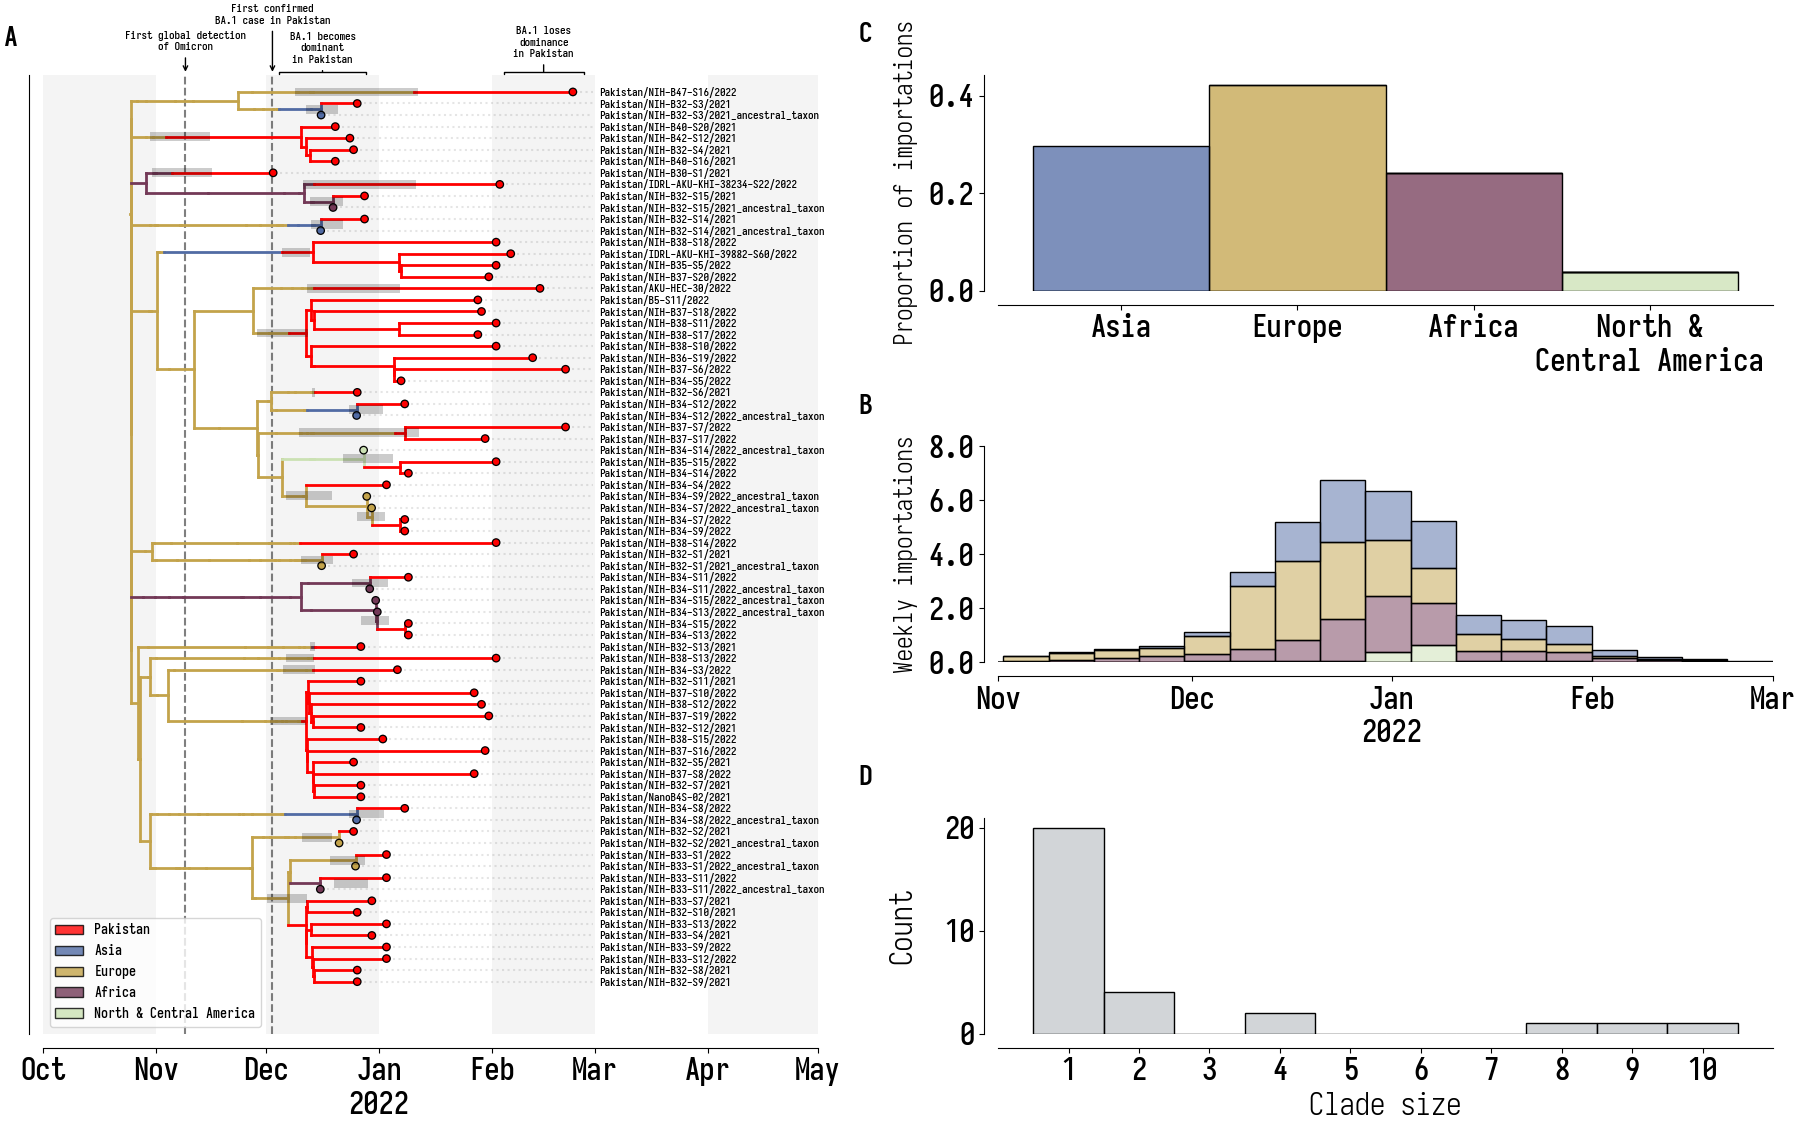
\includegraphics[width=\textwidth]{BA.1_reduced_tree.png}
    \caption{Results of our Bayesian phylogeographic analysis. (A) time-calibrated, reduced maximum clade credibility phylogenetic tree where all taxa from non-Pakistan (or travel history) locations have been hidden. Branches along the tree remain colored by the inferred region of the ancestral strain. Three large Pakistani clades cumulatively representing roughly half of the Pakistani sequences considered in this analysis. (B) distribution of importations to Pakistan by region. (C) Distribution over time of the inferred number of weekly importations to Pakistan, divided by inferred source. (D) individual Pakistani clade count distribution in the MCC tree; most clades are inferred as singletons, representing roughly half of the sequences in the tree.}
    \label{fig:phylogeography}
\end{figure*}

When we subdivide our results by the UN geoscheme subregion, we find that all migrations from Europe (mean estimate $14.81$ migrations) came from Northern Europe (Fig.~\ref{fig:sankey}).
We find that the origin of introductions from Asia is inferred to be split between Western Asia ($8.16$) and Southern Asia ($2.27$), and that the origin of migrations from Africa is split between Eastern Africa ($5.28$), Southern Africa ($1.75$), and Middle Africa ($1.39$).
Finally, we infer Northern America to be a minor source of BA.1 migration into Pakistan (mean estimate $1.32$ migrations).
Of the large Pakistani clades, we find that the three largest were all seeded from Northern Europe (Fig.~\ref{fig:phylogeography}), and the fourth largest was seeded from Western Asia.
Our analysis finds a larger degree of uncertainty in the location of onward BA.1 migrations from Pakistan. However, this uncertainty only applies to the estimated $1.42$ onward transition events (Fig.~\ref{fig:sankey}), which we estimate were most likely to lead into Northern Europe, with regions of China accounting for the majority of additional uncertainty.

\begin{figure*}[ht]
   \centering
   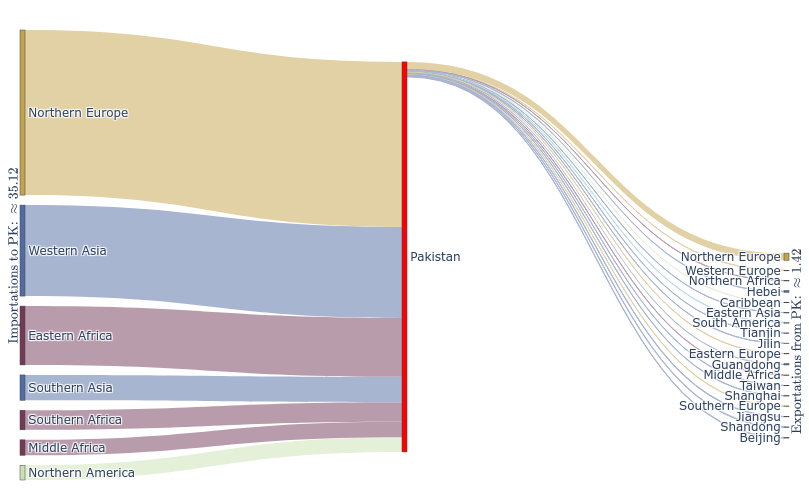
\includegraphics[width=.9\textwidth]{sankey.png}
    \caption{Sankey diagram illustrating inferred BA.1 migrations into (mean estimate $35.12$ migrations) and out of (mean estimate $1.42$ migrations) Pakistan. Northern Europe is the source of all inferred migrations to Pakistan from Europe, representing a plurality of importations from both a region and sub-region geographic resolutions.}
    \label{fig:sankey}
\end{figure*}

We infer with very high probability ($ \geq 0.99$) that the most recent common ancestor of the sequences in our dataset is Northern Europe.
We investigated routes by which BA.1 entered Pakistan by tracing each Pakistani taxon's ancestral history from its final location (Pakistan) backwards in time to the root of the phylogeny (Suppl.~Figs.~\ref{sfig:prov0}--\ref{sfig:prov3}).
We found that, besides direct importation from Northern Europe to Pakistan, the lineages imported from non-European locations were first caused by initial importations from Northern Europe into secondary locations before their dispersal into Pakistan (Fig.~\ref{fig:map}).

We profiled the mutational patterns associated with the Pakistani BA.1 sequences that were included in our Bayesian phylogeographic analysis (Fig.~\ref{fig:mutations}).
While most mutations we observed relative to the reference sequence (MN908947.3) were shared by all Pakistani sequences and are representative of BA.1, we did find several mutations that identify observed large Pakistani clades.
Sequences in of the large clades of Pakistani sequences carry three unique mutations in ORF1a, two not associated with amino acid mutations at sites 3241 and 5914, as well as a a mutation at site 5924 resulting in the ORF1a:V1887I amino acid mutation.
Five sequences from the same clade also contain the S:701V mutation.
The other large Pakistani clade contains sequences that harbour the ORF1b:G1093S and S:R346K mutations, both of which eppear elsewhere in the phylogeny as well.
Finally, among Pakistani sequences we identify ORF3a:L41F as a mutation that appears as polyphyletic within our MCC tree. 


\begin{figure*}[!ht]
    \centering
    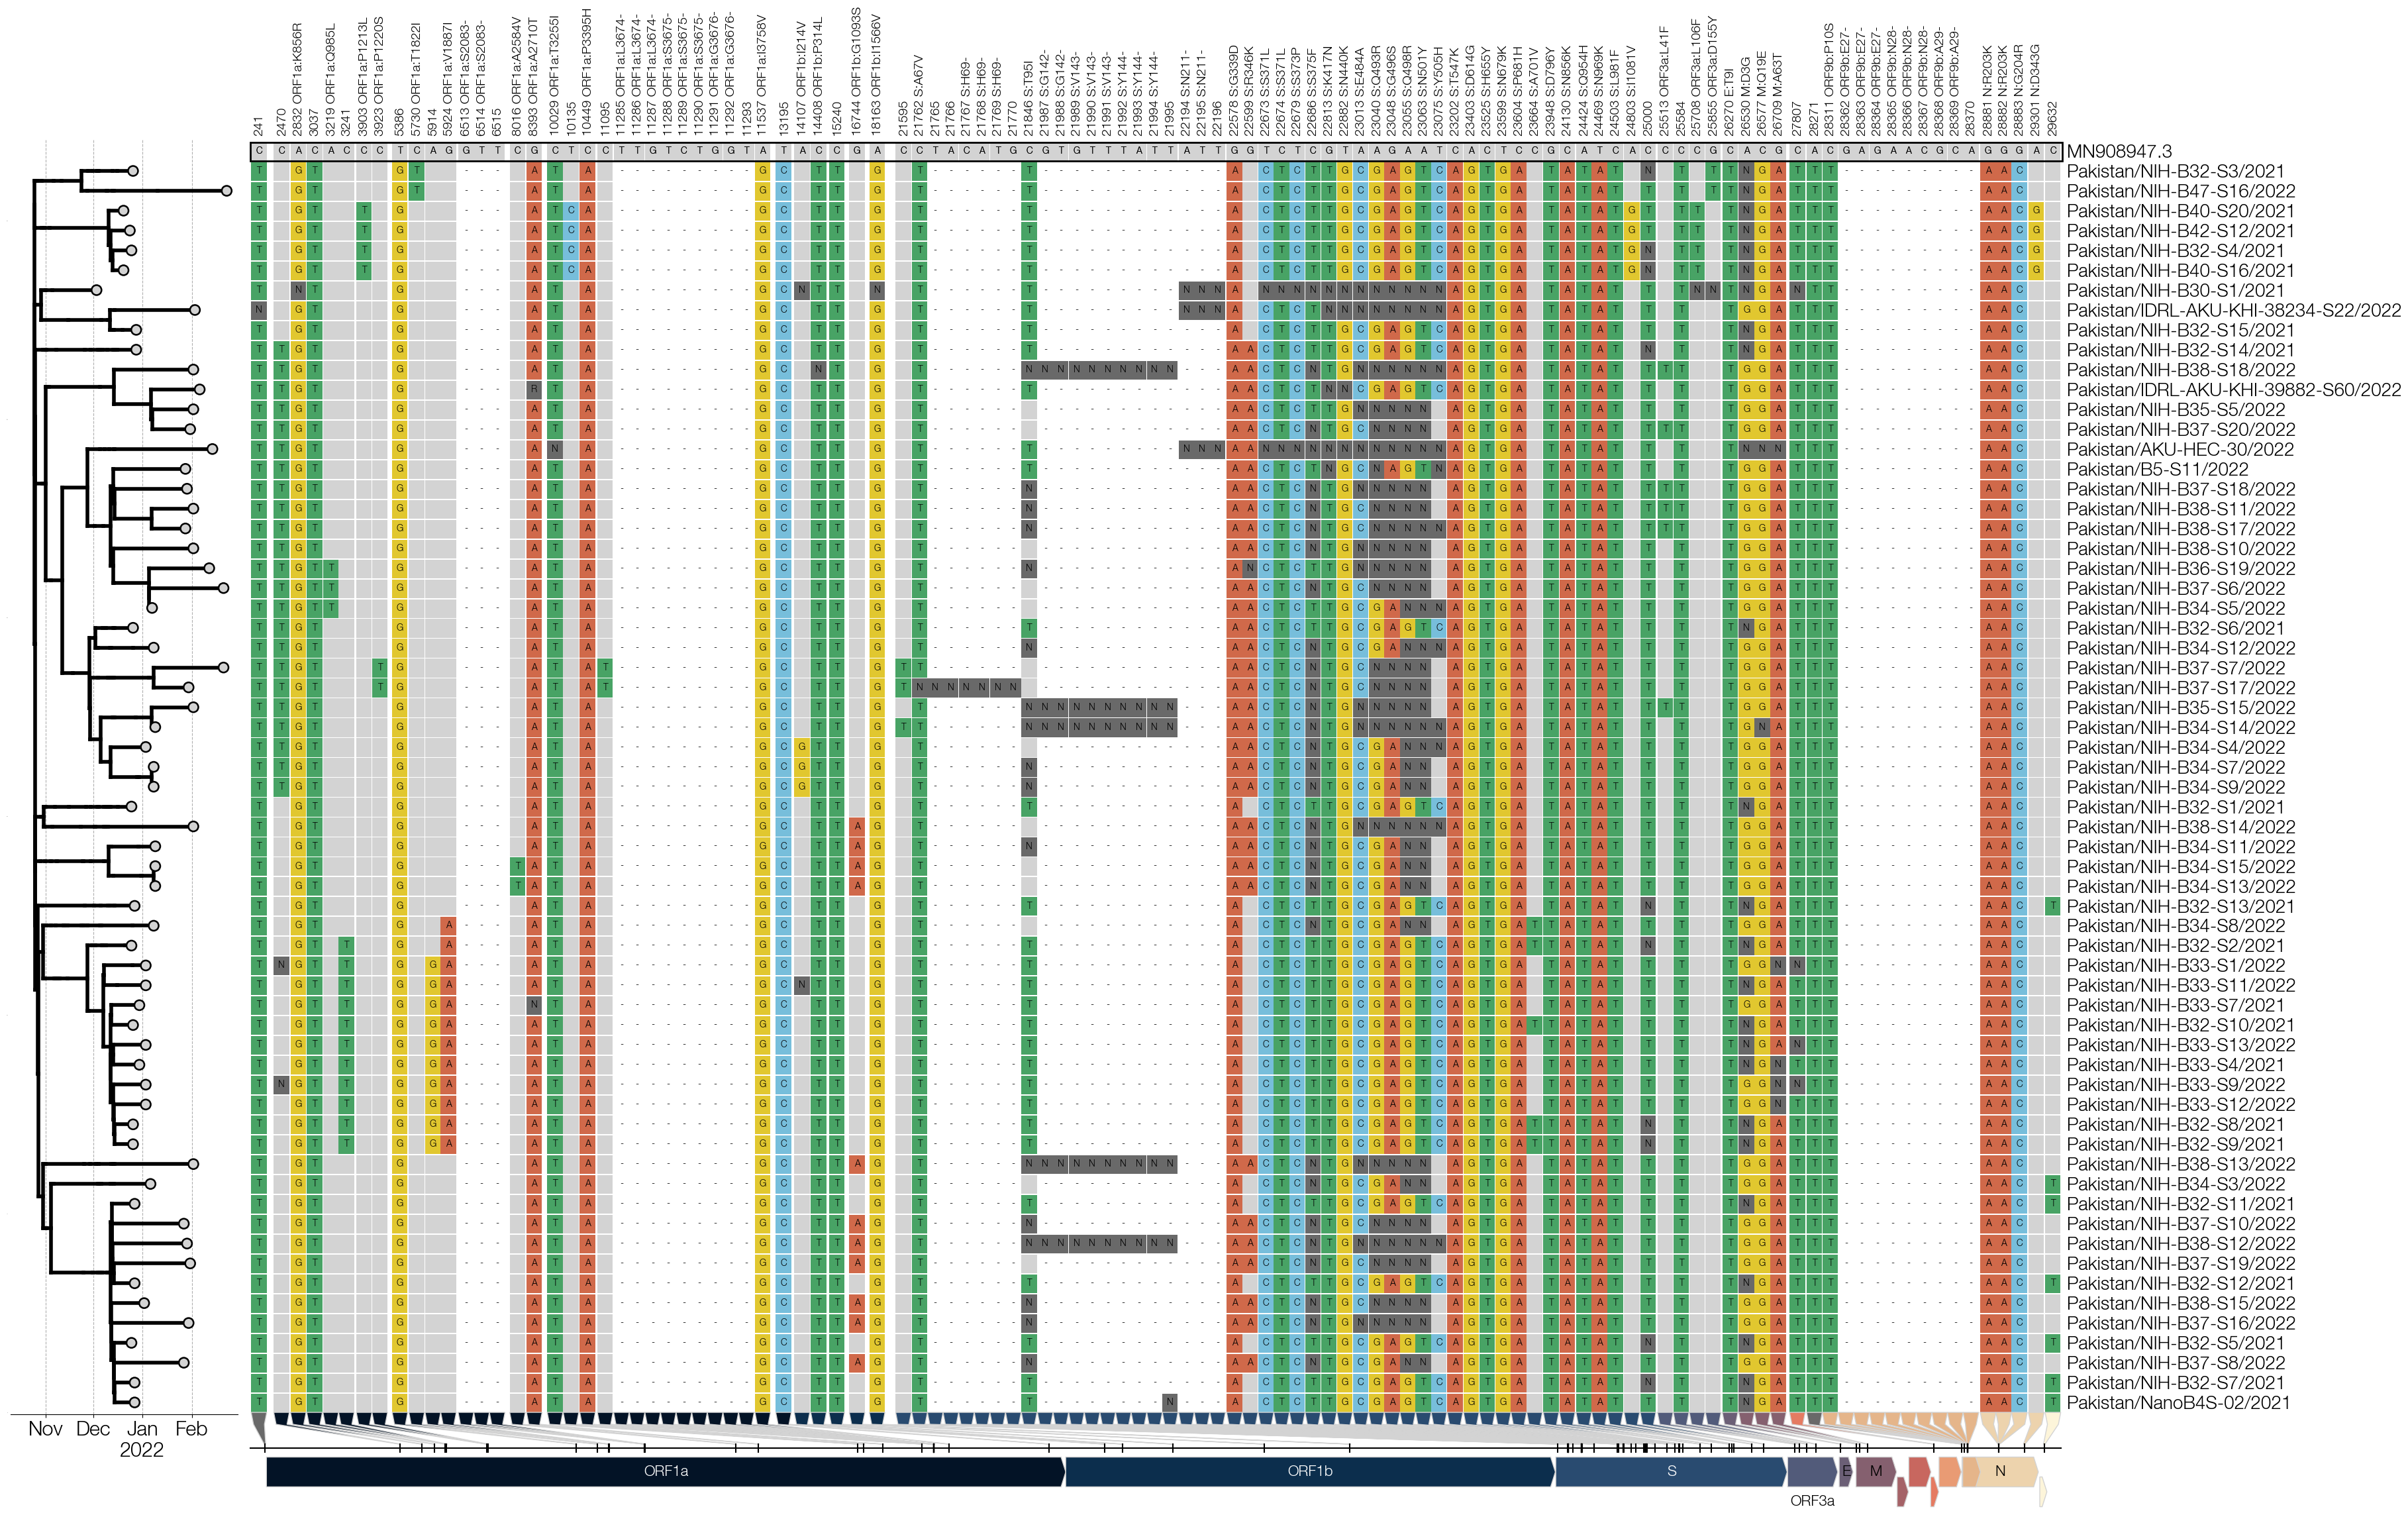
\includegraphics[width=\textwidth]{mutations.png}
    \caption{Condensed alignment of SARS-CoV-2 BA.1 sequences from Pakistan showing sites that are polymorphic within the Pakistan BA.1 dataset and shared by at least two sequences from Pakistan. The tree on the right is based on the MCC tree but is reduced down to just the BA.1 sequences from Pakistan while preserving their relative phylogenetic positions.}
    \label{fig:mutations}
\end{figure*}

\begin{figure*}[ht]
   \centering
   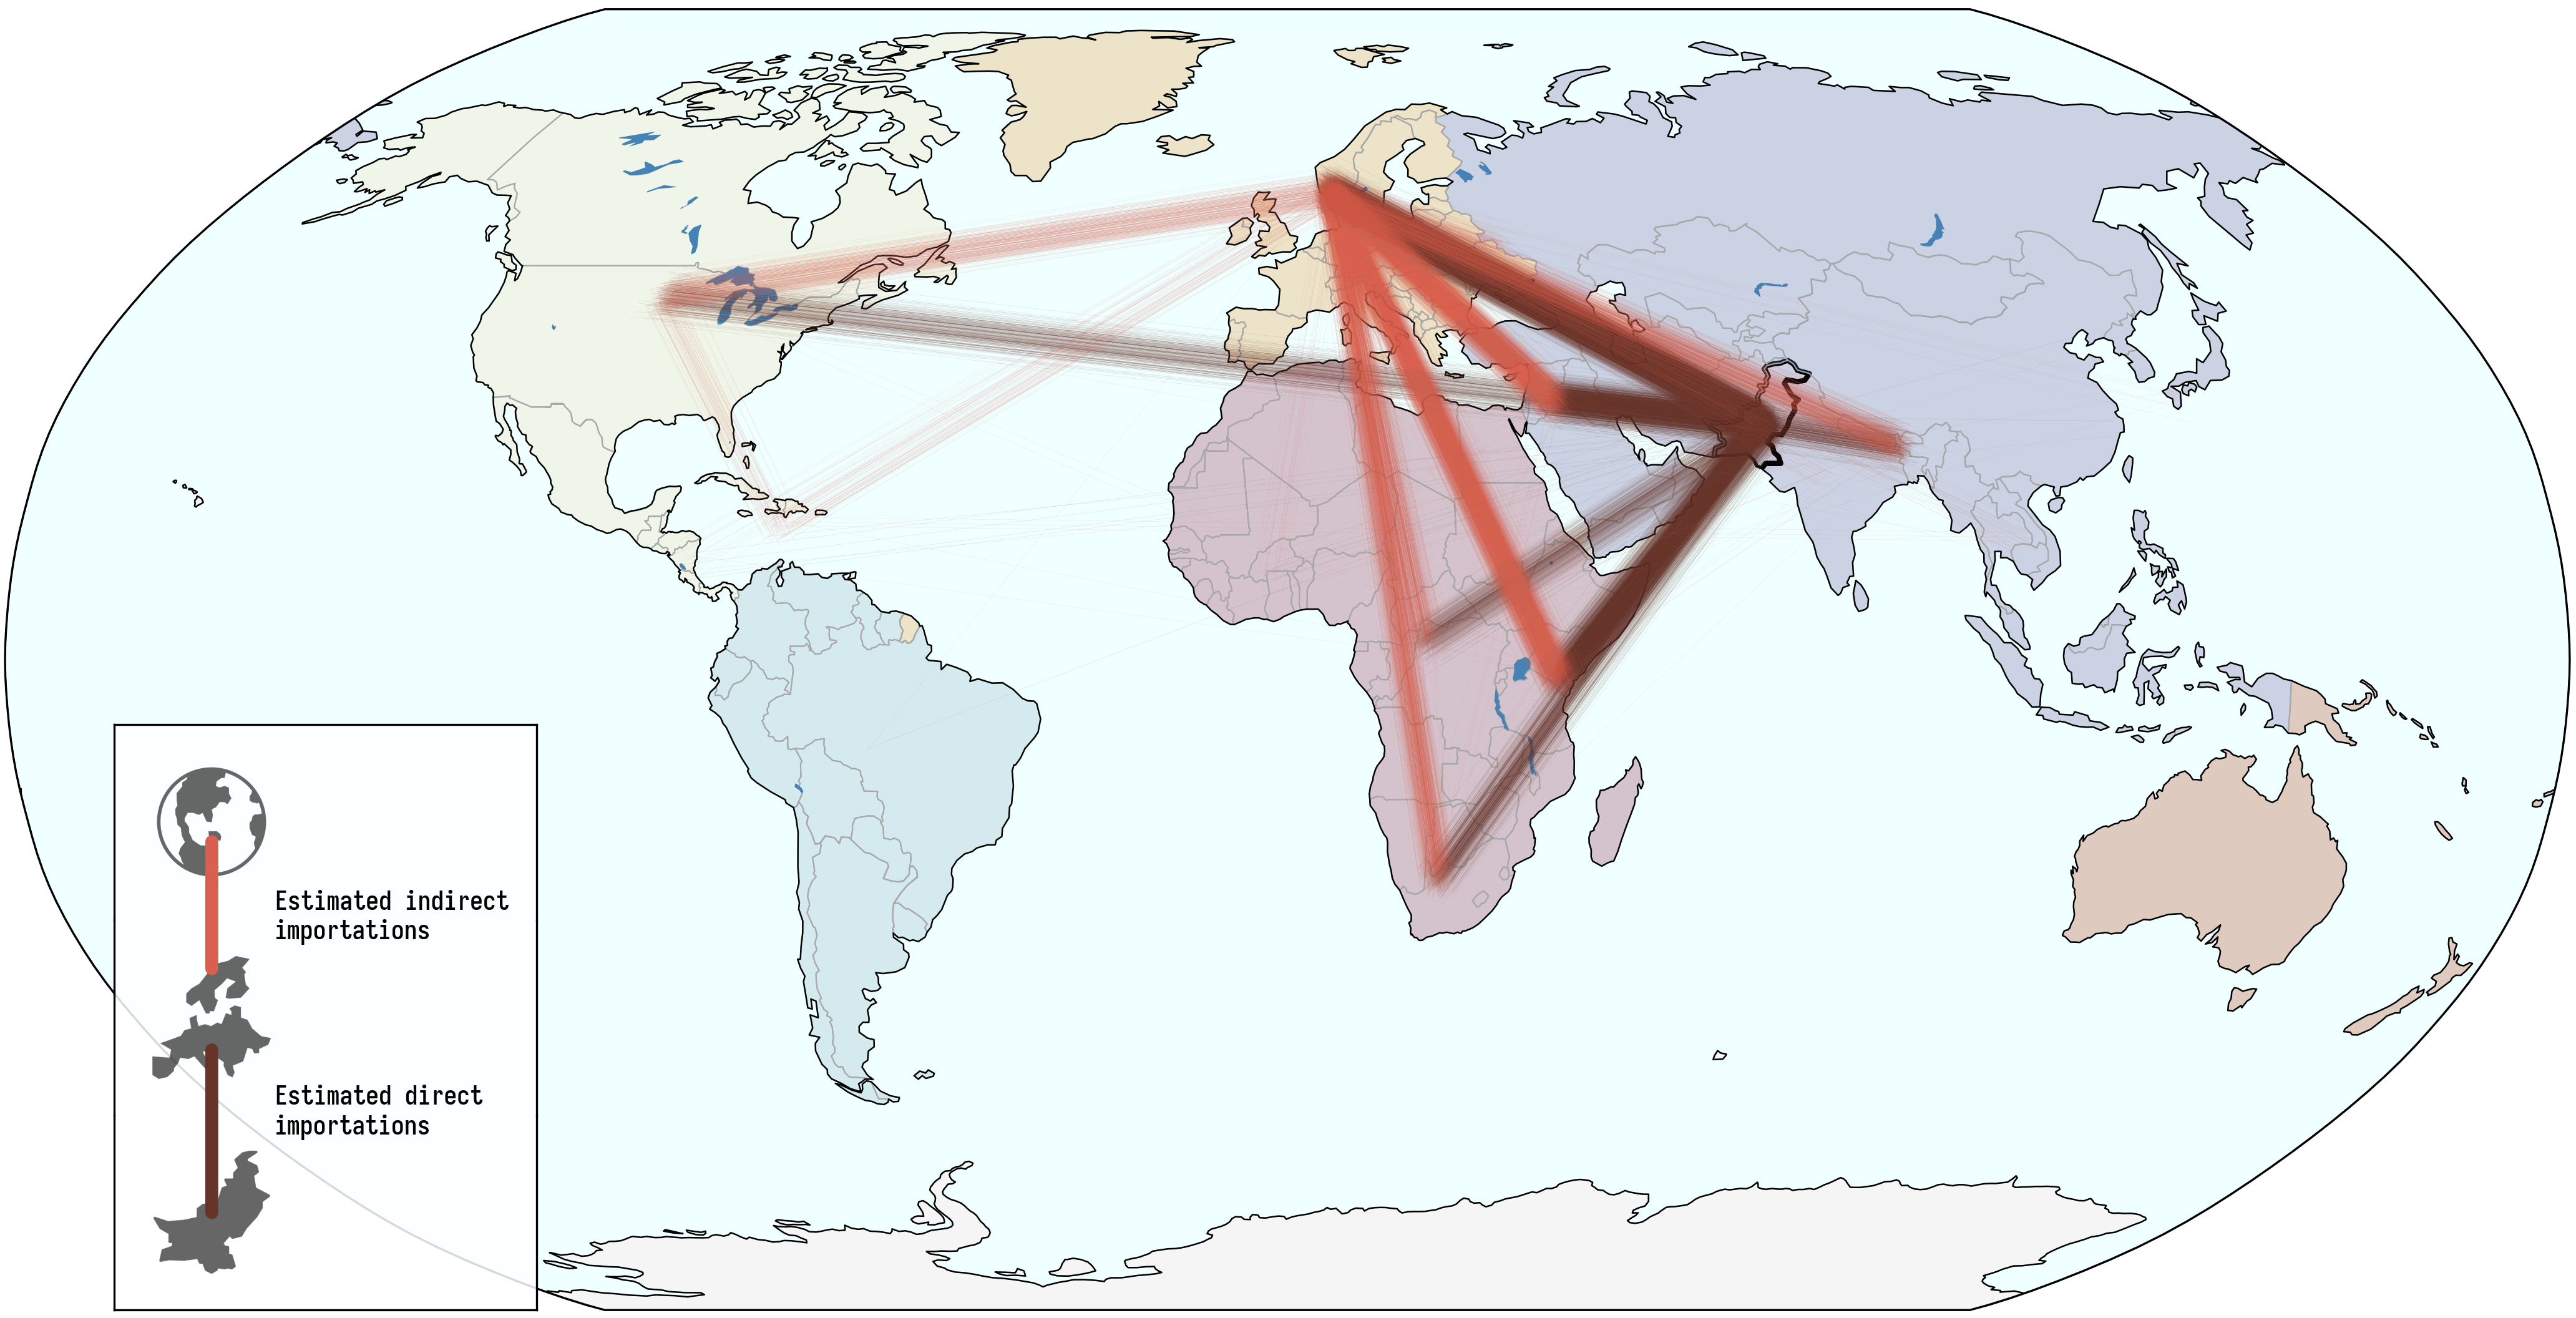
\includegraphics[width=.9\textwidth]{posterior_routes_to_pk.png}
    \caption{Map representing routes by which BA.1 is inferred to enter Pakistan tracing from the most recent common ancestor of our dataset to Pakistani taxa. Inferred migration events that lead directly into Pakistan are represented in dark red, while migrations to a location other than Pakistan that then seed a downstream importation to Pakistan (indirect importations) are illustrated in lighter red.}
    \label{fig:map}
\end{figure*}


\section{Discussion}\label{sec-disc}
BA.2 and its sublineages---also called the ``stealth'' variant---proved difficult to detect by laboratories through PCR when compared to BA.1 and its sublineages.
This was due to the lack of the characteristic S69/70 deletion in BA.2 (targeted by a commercial PCR kit) that halted its rapid identification in clinical samples and affected tracking of the spread of the variant.
Although whole-genome sequencing of SARS-CoV-2 played a central role in the detection and monitoring of the spread of variants during the pandemic, it was primarily limited to specialized facilities having next-generation sequencing equipment, bioinformatics setup, trained human resources and financial resources. These limitations significantly impacted the ability of such genomic methods to be applied in lower-income countries that lacked funding and infrastructure for large-scale genomic analysis.
We developed a PCR-based algorithm and successfully used it for the rapid detection of BA.2, providing an economical solution for the diagnosis and surveillance of this variant in resource-limited settings.

The fifth wave of COVID-19 in Pakistan spanned over three months starting in the last week of December 2021 and ending in the last week of March 2022.
Our curated selection of 1\,642 genotyped and 163 sequenced samples provide critical insights into the temporal, geographic, and phylogenetic distribution of circulating lineages of SARS-CoV-2 in Pakistan from December 2021 to April 10, 2022.
For three months starting in the last week of December 2021 and ending in the last week of March 2022, the fifth wave had 230\,184 cases with a peak ($n=8,183$) detected on January 27, 2022 and the highest positivity ($13\%; n=7,586$) on January 22, 2022.
Before the fifth wave, the genomic surveillance of SARS-CoV-2 showed that the fourth wave of COVID-19 (June--November 2021) in Pakistan was predominated by the Delta variant. However, our results confirm that the fifth wave was caused by Omicron and that Omicron completely replaced Delta extremely quickly after its arrival in Pakistan, owing to its high transmissibility over the Delta variant.
This coincided with the globalization of Omicron and its associated worldwide replacement of Delta \cite{mohapatra2022twin, mohapatra2022Omicron}.

During the study period, according to whole-genome sequencing data ($n=163$), BA.1 (incl. sublineages) was predominant in December, causing 100\% of observed infections, followed by 59\% of cases in January, 20\% in February, and no reported cases thereafter.
On the contrary, no case of BA.2 was reported in December, but it started increasing exponentially from January (41\% of cases) to February (80\%).
BA.2 and its sublineages were completely dominant in March ($BA.2=97\%; BA.2.2=3\%$) and April 2022 ($BA.2=93\%; BA.2.1=7\%$).
These findings are consistent with the trends in cases in Denmark, England, India, the Philippines, and South Africa, where Omicron strains were predominantly sublineage BA.1 in the early stages of the outbreak, and later sublineage BA.2 became predominant \cite{hodcroft2021covariants}.
Interestingly, as in line with the previous reports \cite{mahase2022covid1, mahase2022covid2}, our data also suggest that the driving factor behind the start of the fifth wave was BA.1 (including sublineages) and not BA.2 (including sublineages) in Pakistan.
On 23 February 2022, the UK Health Security Agency (UKHSA) reported, with high confidence, that BA.2 had a substantial growth rate advantage compared to BA.1\cite{ukhsa-risk-assessment}.
On the other hand, our results showed an increase in BA.2 cases but it did not correlate with COVID-19 cases reported at the national level. 
According to the Ministry of National Health Services Regulations and Coordination, Pakistan, a total of 10\,679 cases of COVID-19 were reported in December, 134\,458 in January, 79\,814 in February, 14\,439 in March, and 2\,860 in April.
Our findings are also in agreement with national SARS-CoV-2 genomic surveillance data submitted on GISAID.

The BA.2 (sub)lineages that we sequenced showed 28 unique mutations not shared by our BA.1 (sub)lineage sequences.
In the case of other variants of SARS-CoV-2, the sublineages differ in terms of only one or two mutations but BA.2 harbors relatively more mutations while being considered a subvariant.
These mutations take a toll, with a probable reduction of the immunity in vaccinated as well as already infected individuals.
Moreover, these mutations give the Omicron variant the ability to evade convalescent plasma and monoclonal antibodies \cite{ai2022antibody, altarawneh2022effect}.
In our study, the mutation profile of eight BA.1 isolate shows the absence of S375F, Q498R, N501Y, and Y505H mutations.
However, in comparison with the global sequences on GISAID, the Q498R, N501Y and Y505H mutations are present in 85--87\% of sequences while S375F mutation is present in 93\% of BA.1 and BA.1.1 sequences as of April 30, 2022 \cite{shu2017gisaid}.
Furthermore, in the case of BA.2, there is an absence of Y505H in 42 study isolates but this mutation is observed in 90\% of worldwide reported sequences of BA.2 as of April 30, 2022\cite{shu2017gisaid}.
It had been reported that Q498R and N501Y mutations can increase the binding affinity of spike protein with human ACE2.
These mutations can impact antibody neutralization and vaccine efficacy \cite{schubert2022human}.
The Y505H mutation in the receptor-binding domain resulted in increased binding interactions of Omicron with ACE-2 \cite{ortega2021Omicron}.
The absence of these mutations in the circulating strains of BA.1.1 and BA.2 in the Pakistani population and a recent decline in the number of cases from the fifth wave in Pakistan can be linked to these circulating sub-variants being not
very highly transmissible as the BA.1 and the BA.2 with the Q498R, N501Y, and Y505H mutations.

Notably, we find three significant, rare mutations, F643L (BA.1.17.2), A701V (BA.1.17.2) and T76I (BA.1.13).
The mutations, F643L and A701V are present near the S1/S2 cleavage site and are associated with enhanced fusogenicity and pathogenicity \cite{saito2022enhanced}.
Mutation T76I, located in the N-terminal domain (NTD) region, was observed to affect antibody binding efficiencies and contribute to evading immune response \cite{ou2022tracking}.

In the comparison of the BA.2, BA.1, and BA.1.1 transmissibility, our findings, also corroborated by prior investigations \cite{qassim2022effects, lentini2022monitoring, kirsebom2022covid}, showed that BA.2 had lower mean Ct values ($\approx21$) than BA.1 ($\approx22$) and BA.1.1 ($\approx23$), indicating that BA.2 infections are more recent and/or that higher viral loads contribute to greater transmissibility.
It is necessary to ascertain not just the transmissibility of Omicron sublineages, but also the effectiveness of vaccines.
It is worth noting that numerous studies have proclaimed vaccines to be highly effective at preventing serious illnesses. %GB: citations??
However, it is also clear that the antibody response induced by these vaccines is transient, which leads to breakthrough cases \cite{haque2022mitigating, bruel2022serum, seaman2022vaccine}.
A large number of breakthrough cases of sequenced individuals infected with BA.2 ($74.5\%, n=44$) are identified in the current study.
Of particular concern, by comparing the time intervals between testing positive for BA.1, BA.1.1, or BA.2 after being fully vaccinated, fewer cases are seen within 3 months as compared to the number of cases between 3--6 months after being vaccinated or more than 6 months after being vaccinated.
This result ties well with a prior study where Khoury et al. 2021 \cite{khoury2021covid} demonstrated that antibody titers rose 24-fold after one month of the second dose of vaccine compared to day 1 of the second dose.
A similar pattern of results was obtained in several studies, indicating an elevated antibody titer in the first month after vaccination, a boost in immunity between the first and third months, followed by a steady decrease after three months \cite{chemaitelly2021waning, levin2021waning}.
Conclusively, these findings imply robust immunity for roughly a month, followed by a steady reduction in immunity.
So far, one- and two-dose vaccines provide significantly less protection than those combined with a booster, as seen by increased rates of reinfections and breakthrough infections observed in several studies \cite{healthline-covid19-vaccines, stasi2022sars}.
Interestingly, in the current study, despite the booster shot of Pfizer or Sinovac, 5 subjects still contracted the virus.
In line with our study, another study reported a high incidence of Omicron infections despite booster vaccination in triple-vaccinated individuals \cite{marking2022high}. 
Their results showed post-booster antibody titers to be similar in those with/without subsequent breakthrough infection along with no observed significant differences in viral load and time to the viral clearance between BA.1, BA.1.1, and BA.2 infected individuals.
While \textit{in vitro} neutralization data suggest similar vaccine-induced neutralizing capacity against BA.1 and BA.2 \cite{evans2022neutralization}.
However, data on the vaccine's efficacy and duration of immunity are limited.

In our study, we detected the Omicron variant in 16 inbound passengers from the United Kingdom, Saudi Arabia, Oman, Turkey, South Africa, USA, Ethiopia, and Maldives.
The detection of viruses in travelers highlights the importance of increased testing at all national entry points, as travelers are the major source of introductions of new variants into the community.
Apart from air travel, Pakistan has borders with India, Iran, and Afghanistan which see high levels of pedestrian travel daily.
This amount of foot traffic necessitates increased surveillance not only at ports-of-entry, but also at pedestrian border crossings.
A travel advisory of the civil aviation authority went into effect starting on April 1, 2022, which increased testing at all entry-points for all passengers who presented a valid vaccination card \cite{caapakistan-covid-guidelines}.
However, Rapid Antigen Test (RAT) testing was implemented at each major airport in Pakistan starting May 13, 2022, to screen inbound passengers \cite{brecorder-inbound-flights}.
Examining pedestrian movement across borders, according to NCOC data, between January--April, 2022, 317\,435 passengers crossed the border and among them, 314 ($0.1\%$) were found to be positive.
This low positive number is attributed to reduced testing at the entry points compared to other points-of-entry into Pakistan (unpublished).
The border checkpoint surveillance---particularly at land border checkpoints with Iran and Afghanistan---is limited due to the movement of very large numbers across the border on daily basis, which needs to be expanded to have a more realistic surveillance mechanism for COVID-19.
For the effective control of COVID-19 variants in the future, Pakistan needs to implement mandatory testing along with target sequencing of all inbound travelers entering the country through land and other ports of entry.

With the decline in daily cases, COVID-19 testing not only dropped at points-of-entry, but a global decline in testing was also observed after March 2022.
The overall testing of incoming travelers dropped not only in Pakistan but also in other countries (USA, UK, and India) as well.
There is about a 60\%--75\% decrease in testing since the last COVID-19 waves in these countries \cite{ourworldindata-covid-explorer}.
This low testing is attributed to the difficulty in monitoring the pandemic and tracking the evolution of the virus and its spread.
Due to less number of COVID-19 cases reported, many countries have lifted the restrictions.
Pakistan also lifted all the restrictions following March 17, 2022 \cite{business-standard-covid-curbs}.
Further, restrictions were also eased in countries, United Kingdom \cite{bbc-health-news} and USA \cite{cdc-mask-travel-guidance} where wearing a face mask is no longer mandatory.
Apart from wearing masks and maintaining social distancing, comprehensive vaccination campaigns represented the most effective means to reduce the spread and severity of SARS-CoV-2.
The World Health Organization has strongly recommended improved vaccination rates in all countries \cite{who-covid19-vaccine-advice}.
Up to July 04, 2022, 58\% of the total eligible population of Pakistan was fully vaccinated, 62.6\% was partially vaccinated and 11.8\% had been given boosters.

We investigated the earliest origins of the Omicron variant in Pakistan using travel-history informed Bayesian phylogeographic inference.
Our results suggest that even at the time of its initial detection, the Omicron (BA.1) variant had globalized to some degree, as we infer that it had already entered Pakistan at least twice by that time.
We also find that the greatest force of importation of Omicron into Pakistan was likely seeded from Northern Europe, with importations from neighboring countries not contributing significant numbers of importations into the country.
This suggests that one of the most important factors to controlling the early cases of Omicron, and therefore the severity of its fifth wave of COVID-19, was travellers entering the country via flights from abroad.
As future variants of SARS-CoV-2 and comparable respiratory pathogens emerge this may suggest that increased screening at airports may represent the most efficient use of resources to identify and control incoming variants.
Based on our analyses, we do not identify Pakistan as a major driver of onwards proliferation of the BA.1 variant to other countries.

We infer a roughly equal distribution of sequences that were part of large within-Pakistan clades versus one-off cases that were not closely related to other Pakistani sequences.
This further suggests that a significant portion of the early Omicron wave in Pakistan was driven by returning travelers who did not go on to further drive larger chains of viral transmission, a ratio that mirrors previous finding for the Apha variant \cite{nasir2022evolutionary}.
This result should, however, be interpreted with caution, as there could be a large number of unsampled individuals (either due to systematic difficulties in sampling or infection chains that led to sub-clinical or cryptic transmission of lineages) that may have been related to sequences that we identify as ``singletons''. 
Additionally, as our study period takes place during the inflection point between BA.1 and BA.2 dominance in Pakistan, the competitive advantages of BA.2 over BA.1 could result in a relative muting of BA.1 clade growth, meaning this observation may not be broadly applicable to future SARS-CoV-2 variants that enter Pakistan.

It is important to note that Pakistan represents a setting with relatively limited resources for genomic surveillance compared to other nations.
This results in several important implications for both this study, and for future public health interventions.
Despite its large population of over 240\,000\,000 inhabitants, Pakistan represents less than 1\% of the sequences available on GISAID.
This relative dearth of sequences is reflective of a global trend in which low- and middle-income countries are able to sequence SARS-CoV-2 as a part of a genomic surveillance program at a rate much lower than that of high-income countries \cite{brito2022global}.
As a practical matter, this creates discrepancies in sampling that can significantly bias discrete phylogeographic inference \cite{layan2023impact}.
To mitigate these sampling issues, we have used a bespoke sampling scheme in an attempt to normalize the spatiotemporal sampling of sequences that we use in our analysis.
With the addition of the travel-history data that we incorporate into our analysis, we have used the best-available methodology for reducing biases associated with sampling disparities.
However, it is important to note that our inference of the number of introductions to Pakistan should be interpreted as a lower-bound that represents our best estimate based on the sequence data available.

Furthermore, our results underscore the need for these global disparities in genomic surveillance to be addressed as quickly as possible as a matter of both national and global public health importance.
Within Pakistan, we see that the majority of sequences considered in this study were collected in the capital, Islamabad (Suppl.~Table~\ref{tab:travel_histories}).
With increased genomic surveillance capacity in other regions---and at the locations of important land-border crossings---it may be possible to further refine the inference of the modalities by which future SARS-CoV-2 lineages (and comparable respiratory pathogens) enter the country.
Such an increase in genomic surveillance equity would facilitate more effective public health interventions moving forward into the future, and hopefully reduce the impact of future COVID-19 waves in Pakistan.

%%%%%%%%%%%%%%
\section*{Data availability}
%GB: we should here mention the GISAID IDs of the genomes generated in this study

\section*{Competing interests}
No competing interest is declared.

% \section{Author contributions statement}

% xxxx


\section*{Acknowledgments}
B.I.P. and G.B. acknowledge support from the Internal Funds KU Leuven (Grant No. C14/18/094).
S.L.H. and G.B. acknowledge support from the Research Foundation - Flanders (``Fonds voor Wetenschappelijk Onderzoek - Vlaanderen,'' G0E1420N) and from the DURABLE EU4Health project 02/2023-01/2027, which is co-funded by the European Union (call EU4H-2021-PJ4) under Grant Agreement No. 101102733.
G.B. acknowledges support from the Research Foundation - Flanders (``Fonds voor Wetenschappelijk Onderzoek - Vlaanderen,'' G098321N) and from the European Union Horizon 2023 RIA project LEAPS (grant agreement no. 101094685).



%%%%%%%%%%%%%%%%%%%%%%%%%%%%%%%%%%%%%%%%%%%%%%%%%%
% Keep the following \cleardoublepage at the end of this file, 
% otherwise \includeonly includes empty pages.
\cleardoublepage

% vim: tw=70 nocindent expandtab foldmethod=marker foldmarker={{{}{,}{}}}
